%% -*- coding: utf-8 -*-
\documentclass[14pt,a4paper]{scrartcl} 
\usepackage[utf8]{inputenc}
\usepackage[english,russian]{babel}
\usepackage{indentfirst}
\usepackage{misccorr}
\usepackage{graphicx}
\usepackage{amsmath}
\usepackage{listings}

\begin{document}
\tableofcontents
\newpage
\section{Введение}
Для написания алгоритма сортировки быстрой и слияния  была использована среда разработки online C++ compiler. Для оформления и написания отчёта использовался онлайн-компилятор LaTeX Overleaf


\newpage
\section{Алгоритм решения}
Быстрая сортировка (QuickSort):

QuickSort — это алгоритм сортировки, который обрабатывает весь массив по очереди, выбирая элемент в качестве опорного (pivot) и делит элементы на две подгруппы: те, которые больше опорного, и те, которые меньше опорного. Затем эти подгруппы рекурсивно сортируются.

Алгоритм начинает с выбора элемента в середине массива, называемого опорным (pivot). Затем он ищет элементы слева и справа от опорного элемента, которые нужно поменять местами, и продолжает этот процесс до тех пор, пока левый индекс не станет больше правого. После этого опорный элемент окажется в конечном положении, и массив разделяется на две части. Рекурсивно повторяя этот процесс для каждой из этих двух частей, пока массив не будет полностью отсортирован.

Сортировка слиянием (MergeSort):

MergeSort — это алгоритм сортировки, который разделяет массив на две части и рекурсивно сортирует каждую из них, а затем объединяет (сливает) эти две отсортированные части в один массив.

Алгоритм начинает с разбиения (splitting) массива на две части, путем нахождения средней точки (mid). Затем сортируются две новые части массива с помощью рекурсивного вызова MergeSort. Когда обе части отсортированы, они объединяются (merge) в один отсортированный массив. Для объединения двух отсортированных массивов используется процедура слияния (merge), которая сравнивает два элемента из разных массивов и помещает наибольший из них в новый массив.

Главное отличие между QuickSort и MergeSort заключается в том, что QuickSort разделяет массив на месте, тогда как MergeSort использует дополнительную память для разделения массива. QuickSort является более быстрой, но менее стабильной сортировкой, в то время как MergeSort более устойчивая, но медленнее работает.Быстрая сортировка (QuickSort):

QuickSort — это алгоритм сортировки, который обрабатывает весь массив по очереди, выбирая элемент в качестве опорного (pivot) и делит элементы на две подгруппы: те, которые больше опорного, и те, которые меньше опорного. Затем эти подгруппы рекурсивно сортируются.

Алгоритм начинает с выбора элемента в середине массива, называемого опорным (pivot). Затем он ищет элементы слева и справа от опорного элемента, которые нужно поменять местами, и продолжает этот процесс до тех пор, пока левый индекс не станет больше правого. После этого опорный элемент окажется в конечном положении, и массив разделяется на две части. Рекурсивно повторяя этот процесс для каждой из этих двух частей, пока массив не будет полностью отсортирован.

Сортировка слиянием (MergeSort):

MergeSort — это алгоритм сортировки, который разделяет массив на две части и рекурсивно сортирует каждую из них, а затем объединяет (сливает) эти две отсортированные части в один массив.

Алгоритм начинает с разбиения (splitting) массива на две части, путем нахождения средней точки (mid). Затем сортируются две новые части массива с помощью рекурсивного вызова MergeSort. Когда обе части отсортированы, они объединяются (merge) в один отсортированный массив. Для объединения двух отсортированных массивов используется процедура слияния (merge), которая сравнивает два элемента из разных массивов и помещает наибольший из них в новый массив.

Главное отличие между QuickSort и MergeSort заключается в том, что QuickSort разделяет массив на месте, тогда как MergeSort использует дополнительную память для разделения массива. QuickSort является более быстрой, но менее стабильной сортировкой, в то время как MergeSort более устойчивая, но медленнее работает.
\newpage


\section{Программа}


\begin{figure}[h!]
    \centering
    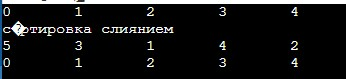
\includegraphics [width=0.9\textwidth]{result}\\
    \caption{Результат выполнения программы}
    \label{fig:picResult}
\end{figure}
\end{document}